\documentclass{article}
\usepackage[left=2cm, right=2cm, top=1cm, bottom=1cm]{geometry}
\usepackage{graphicx}
\usepackage{amsmath}
\usepackage{amssymb}
\usepackage{amsthm}
\usepackage{fancyhdr}
\usepackage{verbatim}
\usepackage{listings}
\usepackage{xcolor}
\usepackage{pgfplots}

\lstset{
    language=C++,
    basicstyle=\ttfamily\footnotesize,
    keywordstyle=\color{blue},
    commentstyle=\color{green},
    stringstyle=\color{red},
    numbers=left,
    numberstyle=\tiny\color{gray},
    frame=single,
    breaklines=true,
    captionpos=b,
}


\title{PHYS 325: Lecture 4}
\author{Cliff Sun}

\newtheorem{theorem}{Theorem}[section]
\newtheorem{lemma}[theorem]{Lemma}
\newtheorem{definition}[theorem]{Definition}
\newtheorem{conjecture}[theorem]{Conjecture}
\newtheorem{proposition}[theorem]{Proposition}
\newtheorem{corollary}[theorem]{Corollary}
\newtheorem{one minute paper}[theorem]{One Minute Paper}

\pagestyle{fancy}
\lhead{\textbf{\thepage}\ \ \nouppercase{\rightmark}}
\chead{PHYS 325: Lecture 4}
\rhead{Cliff Sun}

\begin{document}

\maketitle

\section*{Lecture Span}
\begin{itemize}
    \item Recap (potential curve)
    \item Simple Harmonic Oscillator
    \item Drag Forces
\end{itemize}

\section*{Potential Curves}
To analyze extrema points of potential, all we do is 
\begin{equation}
    \left(\frac{dU}{dx}\right)_{x_0} = 0
\end{equation}
So what happens if we perturb the particle near the extremas?

\subsection*{Minimum}
Check if the 2nd derivative of the potential at the extrema is greater than 0. Than this means that the 
particle is trapped in a local minima, and any perturbations to the particle will result in it settling in the minimum for time sufficiently high. This is called \underline{stable}. 

\subsection*{Maximum}
If the 2nd derivative of the potential is less than 0, then any pertubation will result in the particle leaving the extrema. This is called \underline{unstable}. 

\subsection*{Saddle point}
If the 2nd derivative of the potential at the extrema is 0, then we call the system \underline{marginally stable}, since it may be stable in one direction but not in another. 

\section*{Simple Harmonic Oscillator}
Suppose we're given some graph with a local minima near $x_0$,  

We first taylor expand the potential around $x_0$, that is

\begin{equation}
    U(x) \approx U(x_0) + U'_{x_0}(x-x_0) + \frac{1}{2}U''_{x_0}(x-x_0)^2 + \cdots
\end{equation}

Since we are in an extrema, we know that $U'_{x_0} = 0$, and letting $U''_{x_0} = k$, we obtain
\begin{equation}
    U(x) \approx U(x_0) + \frac{1}{2}k(x-x_0)^2
\end{equation}

We choose $U(x_0) = 0$ and shift our coordinate axis $x' = x + x_0$, we transform the problem to 
\begin{equation}
    U(x)' \approx \frac{1}{2}kx'^2
\end{equation}

Note that this looks like the spring potential. We now solce the following differential equation:

\begin{equation}
    F = ma = m\ddot{x}
\end{equation}


\begin{center}
    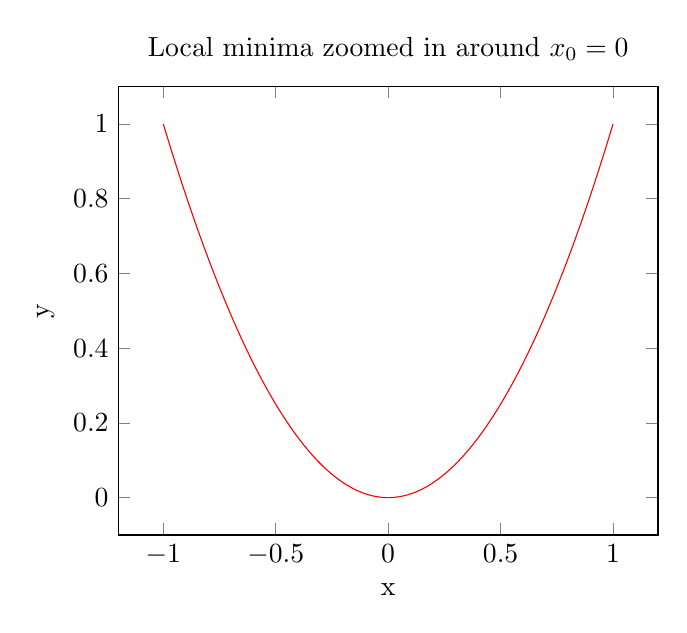
\begin{tikzpicture}
        \begin{axis}[
            title={Local minima zoomed in around $x_0 = 0$},
            xlabel={x},
            ylabel={y}
        ]
            \addplot[color=red, domain=-1:1, samples=100]{x^2};
        \end{axis}
    \end{tikzpicture}
\end{center}

When restricting ourselves to this local minima, we obtain

\begin{equation}
    F(x) \approx F_{x_0} + F'_{x_0}(x-x_0) + F''_{x_0}(x-x_0)^2 + \cdots
\end{equation}

We write $F = -\frac{dU}{dx}$ we write $F_{x_0} = -\frac{dU}{dx}_{x_0} = 0$. Similarly, $F' = k$ we compute this 
\begin{equation}
    F(x) \approx -kx'
\end{equation}
by shifting the coordinate axis $x' = x + x_0$. So we see that
\begin{equation}
    m\ddot{x} = -kx
\end{equation}
or 
\begin{equation}
    m\ddot{x} + kx = 0
\end{equation}
This is the equation for the simple harmonic oscillator. The solution is
\begin{equation}
    x(t) = A\sin(\sqrt{\frac{k}{m}} + \phi_0)
\end{equation}
or 
\begin{equation}
    x(t) = Ae^{i \sqrt{\frac{k}{m}} \ t}
\end{equation}
Where the phase is encoded within the amplitude of the complex solution. Note that the frequency $\omega = \sqrt{\frac{k}{m}}$. 

Note that the period is $\frac{2\pi}{\omega}$

\newpage 

\section*{Drag Forces}

We first note that $\vec{F} = \vec{F}\left(\vec{v}\right)$, or that forces are purely a function of velocity. This could be friction, air resistance, etc. 

\subsection*{Types of Drag Forces}
\begin{enumerate}
    \item Stoke's Drag (linear drag), we describe the drag as 
    \begin{equation}
        F = -cv
    \end{equation}
    Note the minus sign, as it means that the drag acts in the opposite direction of velocity. This includes
    \begin{itemize}
        \item Laminar flow
        \item Very viscous fluids (Honey, etc.)
        \item Small velocities
    \end{itemize}
    \item Newtonian drag (nonlinear), we describe the drag as 
    \begin{equation}
        F = -k v^2
    \end{equation}
    This differential equation can describe turbulent flow. This is valid for 
    \begin{itemize}
        \item Large velocities
        \item Less viscous fluids (e.g. air)
    \end{itemize}
    What type is this applicable?
    \begin{itemize}
        \item Reynold's number: $R_e = \frac{\rho v L}{\mu}$ Where $\mu$ = viscosity and $L$ = size. If this number
        is small (e.g $< 2300$) then we get laminar flow. Else, we get turbulent flow. 
    \end{itemize}
\end{enumerate}

\subsection*{Example 1: Linear Drag}

\subsubsection*{Setup} Particle $m$ and initial velocity $v_0 = v_0 \neq 0$, we derive $\vec{v}(t)$ at late times. 

\subsubsection*{Strategy}
\begin{enumerate}
    \item Choose coordinates: 1D along the $x$ axis, and let $v = \dot{x}$
    \item Force $F(v) = -cv$, we also introduce a new constant $\kappa = \frac{c}{m}$. We rewrite $F = -mkv$
    \item in EOM, we start with N2L, we get 
    \begin{equation}
        m\dot{v} = -mkv \iff \dot{v} = -kv
    \end{equation}
    The solution is 
    \begin{equation}
        v(t) = v_0e^{-kt}
    \end{equation}
\end{enumerate}

\end{document}